%%%%%%%%%%%%%%%%%%%%%%%VICARIOUS%%%%%%%%%%%%%%%%%%%%%%%%%%%%%%%%%%%%%%%
% 																	%
% Template for presentation in Latex`s Beamer Class					%
% Using the default Berlin theme, can be replaced by other themes		%
% logo in the upper right can be replaced by new .png, gif, eps etc	%
% 																	%
%%%%%%%%%%%%%%%%%%%%%%%%%%%%%%%%%%%%%%%%%%%%%%%%%%%%%%%%%%%%%%%%%%%%%%%
\documentclass[xcolor=dvipsnames, aspectratio=169]{beamer}
\usetheme{Berlin}
\usecolortheme[named=LimeGreen]{structure}
\usepackage{beamerthemesplit} % kam neu dazu
\usepackage[ngerman]	{babel}			
\usepackage{t1enc}						
\usepackage[utf8]{inputenc}			
\usepackage{amsmath}
\usepackage{graphicx}
\graphicspath{{pictures/}}
\usepackage{amssymb}
\usepackage{amsfonts}
\usepackage{caption}
\usepackage{multimedia}
\usepackage{tikz}
\usepackage{listings}
\usepackage{acronym}
\usepackage{subfig}

\usepackage{lmodern}
\usepackage{multicol}

\definecolor{pblue}{rgb}{0.13,0.13,1}
\definecolor{pgreen}{rgb}{0,0.5,0}
\definecolor{pred}{rgb}{0.9,0,0}
\definecolor{pgrey}{rgb}{0.46,0.45,0.48}

\lstset{
    escapeinside={(*}{*)}
}

\lstdefinestyle{Java}{
  showspaces=false,
  showtabs=false,
  tabsize=2,
  breaklines=true,
  showstringspaces=false,
  breakatwhitespace=true,
  commentstyle=\color{pgreen},
  keywordstyle=\color{pblue},
  stringstyle=\color{pred},
  basicstyle=\footnotesize\ttfamily,
  numbers=left,
  numberstyle=\tiny\color{gray}\ttfamily,
  numbersep=7pt,
  %moredelim=[il][\textcolor{pgrey}]{$$},
  moredelim=[is][\textcolor{pgrey}]{\%\%}{\%\%},
  captionpos=b
}

\lstdefinestyle{basic}{  
  basicstyle=\footnotesize\ttfamily,
  breaklines=true
  numbers=left,
  numberstyle=\tiny\color{gray}\ttfamily,
  numbersep=7pt,
  backgroundcolor=\color{white},
  showspaces=false,
  showstringspaces=false,
  showtabs=false,
  frame=single,
  rulecolor=\color{black},
  captionpos=b,
  keywordstyle=\color{blue}\bf,
  commentstyle=\color{gray},
  stringstyle=\color{green},
  keywordstyle={[2]\color{red}\bf},
}


\lstdefinelanguage{custom}
{
morekeywords={public, void},
sensitive=false,
morecomment=[l]{//},
morecomment=[s]{/*}{*/},
morestring=[b]",
}


\lstdefinestyle{BashInputStyle}{
  language=bash,
  showstringspaces=false,
  basicstyle=\small\sffamily,
  numbers=left,
  numberstyle=\tiny,
  numbersep=5pt,
  frame=trlb,
  columns=fullflexible,
  backgroundcolor=\color{gray!20},
  linewidth=0.9\linewidth,
  xleftmargin=0.1\linewidth
}

%Logo in the upper right just change if you know what you are doing^^
\addtobeamertemplate{frametitle}{}{%
\begin{tikzpicture}[remember picture,overlay]
\node[anchor=north east,yshift=2pt] at (current page.north east) {
\includegraphics[height=1.8cm]{htw}};
\end{tikzpicture}}

\begin{document}
\bibliographystyle{alpha}
\title{Netzwerke -- Übung SoSe 2019}
\subtitle{IT Security\\
		\href{mailto:Benjamin.Troester@HTW-Berlin.de}{Benjamin.Troester@HTW-Berlin.de}\\
		PGP: ADE1 3997 3D5D B25D 3F8F 0A51 A03A 3A24 978D D673 }
\author{Benjamin Tröster}

\date{}

\begin{frame}
\titlepage

\end{frame}

\section*{Road-Map}
\begin{frame}
\frametitle{Road-Map}
\begin{multicols}{2}
  \tableofcontents
\end{multicols}
\end{frame}

\section{Aktueller Stand}
\begin{frame}
	\frametitle{Aktueller Stand}
	\begin{itemize}
		\item Anwendungsprotokolle und Analyse des Netzwerkverkehrs
		\item Einige ausgewählte Protokolle:
		\begin{itemize}
			\item DNS
			\item HTTP(S)
			\item IMAP, SMTP
		\end{itemize}
		\item Erste Berührungspunkte mit Crypto -- \emph{openssl}
	\end{itemize}
\end{frame}

\section{Kryptografie}
\subsection{Crypto}
\begin{frame}{}
\begin{itemize}
	\item Arten von Chiffren:
	\begin{itemize}
		\item Symmetrische Chiffren
		\begin{itemize}
			\item AES, Towfisch, 3DES, RC2, RC4, RC5, RC6, One-Time-Pad, Serpent, \dots
			\item Unterscheidung in Stromchiffre und Blockchiffre
			\item Verschiedene Verfahren haben unterschiedliche Modi -- CBC, EBC etc.
		\end{itemize}
		\item Asymmetrische Chiffren
			\item RSA, Merkle-Hellman, Diffie-Hellman, ElGamal, \dots
			\item Generierung eines Schlüsselpaars -- private \& public
			\item Funktionsweise aufgrund von mathematisch schwer lösbaren Problemen: Einwegfunktionen
			\item Faktorisierungsproblem, diskretes Exponentiation/Wurzelziehen ($ \sqrt[\leftroot{-2}\uproot{2}\alpha]{n} \mod N$), diskreter Logarithmus, \dots
	\end{itemize}
\end{itemize}
\end{frame}

\begin{frame}
	\begin{figure}
	\center
	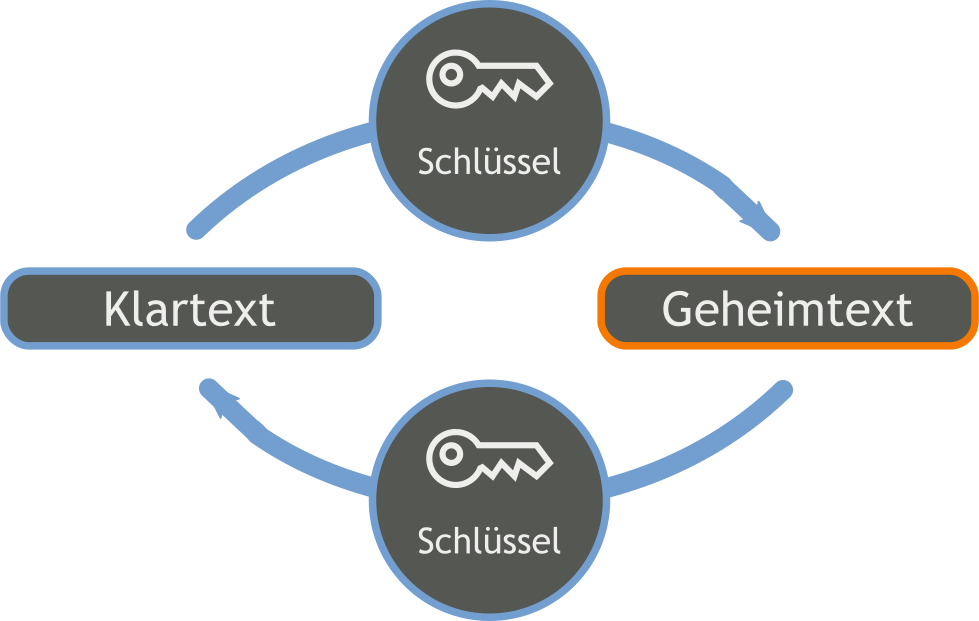
\includegraphics[scale=0.2]{symmetric_cryptography}
	\end{figure}
\end{frame}


\begin{frame}
	\begin{figure}
	\center
	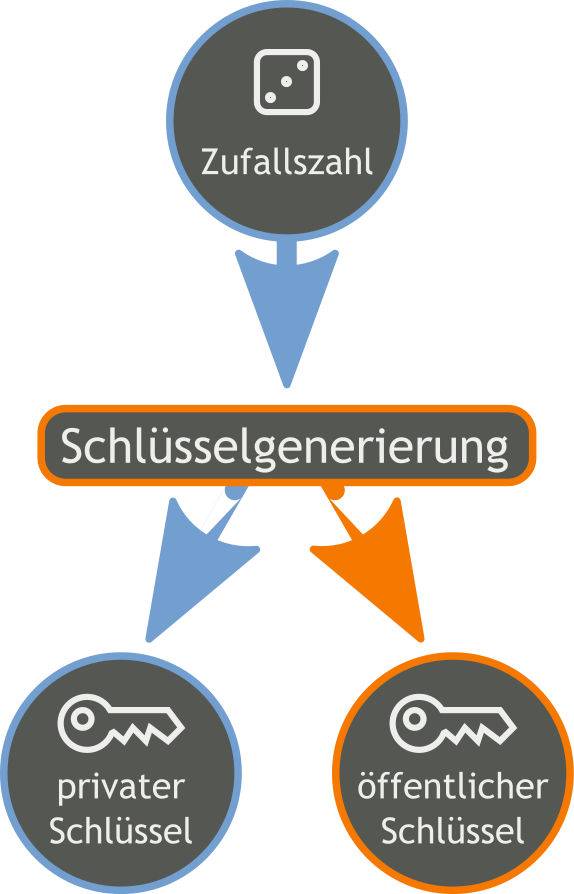
\includegraphics[scale=0.2]{private_keygeneration}
	\end{figure}
\end{frame}
\begin{frame}
	\begin{figure}
	\center
	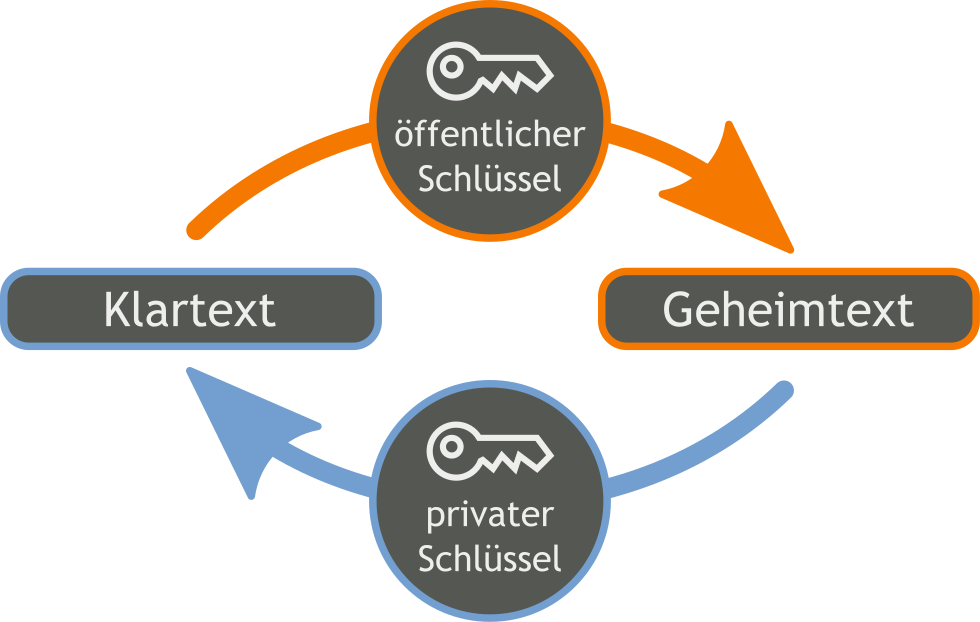
\includegraphics[scale=0.2]{public_key_cryptography}
	\end{figure}
\end{frame}

\begin{frame}
	\begin{figure}
	\center
	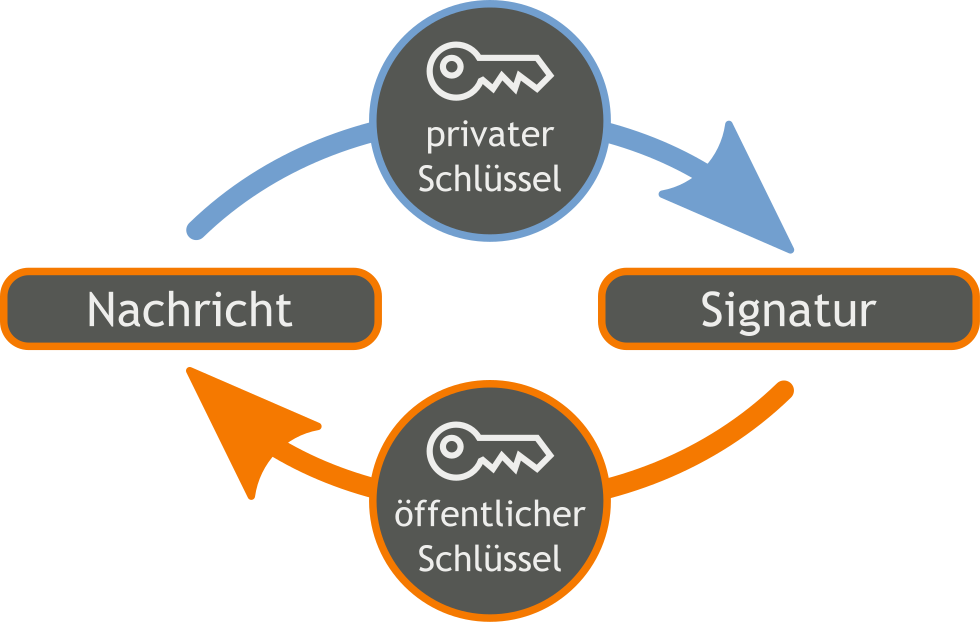
\includegraphics[scale=0.2]{digital_signature}
	\end{figure}
\end{frame}

\subsection{SSH}
\begin{frame}
\centering

\includegraphics[scale=0.5]{ssh}
\end{frame}

\begin{frame}{SSH}
\begin{itemize}
	\item SSH -- Secure Shell
	\item Sammlung von Programmen/Diensten \& Protokolle zur sichere Netzwerkkommunikation
	\item Sicherung der Kommunikation durch:
	\begin{itemize}
		\item Kryptografie
	\end{itemize}
	\item Aufgaben:
	\begin{itemize}
		\item Verschlüsselung der Daten
		\item Integrität von Daten 
		\item Authentizität des Absenders
		\item Autorisierung -- nur Befugte könne die Daten einsehen
	\end{itemize}
\end{itemize}
\end{frame}

\begin{frame}
\begin{figure}
\center
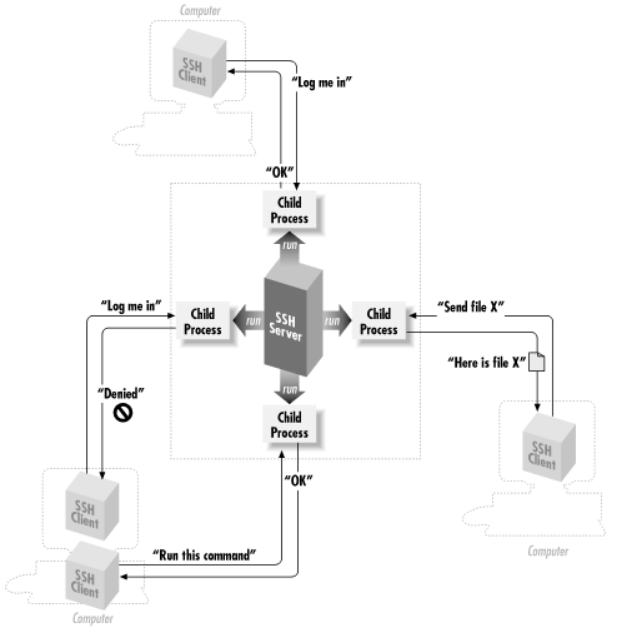
\includegraphics[scale=0.25]{ssh2}
\end{figure}
\end{frame}



\end{document}